\documentclass{article}
% This text is inserted in the beginning of all
% LaTex and Tex files I create.
%
% File created: Thu Apr  1 2010
% File name:    paper.tex
% Path:         /home/mroughan/Reports/Networking/Topology/Waxman/
%
% Matthew Roughan
% matthew.roughan@adelaide.edu.au
%
\usepackage{fancyhdr}
\usepackage{epsf}
\usepackage{subfig}
\usepackage{latexsym}
\usepackage{dsfont}
\usepackage{url}
\usepackage{times}
\usepackage{graphicx}
\usepackage{amsfonts}
\usepackage{amsmath}
\usepackage{ifthen}
\usepackage{verbatim}

\setlength{\headheight}{10mm}
\setlength{\headsep}{10mm}
\setlength{\topmargin}{0cm}
\setlength{\textwidth}{175mm}
\setlength{\textheight}{225mm}
\setlength{\oddsidemargin}{-10mm}
\lefthyphenmin=2
\righthyphenmin=3

\renewcommand{\baselinestretch}{1.0}
\renewcommand{\textfraction}{0.1}


\def\RR{\mathds{R}}
\def\CC{\mathds{C}}

\newcommand{\titlestr}{Known Results for the Line Picking Problem}
\rhead[]{{\small \titlestr}}
\lhead[{\small }]{}
\cfoot{}
\rfoot[]{{\rm\thepage}}
\lfoot[{\rm\thepage}]{}
\renewcommand{\footrulewidth}{0.4pt}
\pagestyle{fancy}

\newtheorem{theorem}{Theorem}[section]
\newtheorem{lemma}{Lemma}[theorem]
\newtheorem{corollary}[theorem]{Corollary}
\newtheorem{Def}{Definition}[section]


\begin{document}
\title{\titlestr}
\author{Matthew Roughan \;\;\; Eric Parsonage \;\;\; Jonathon Tuke \\
 School of Mathematical Sciences \\
 University of Adelaide \\
 \url{ <{matthew.roughan,eric.parsonage,}@adelaide.edu.au> } }
\maketitle

\begin{abstract}

\end{abstract}

\section{Introduction}

The {\em line picking} problem is a standard problem in stochastic
geometry, where we pick lines at random from some region. The typical
questions one asks are what will then mean line length be? What will
the Probability Density Function (PDF) be?

This brief note describes the current list of known PDFs, and where
they were derived, as well as the current set of code to calculate
these. 

The code is written in C with minimal external dependencies, and with
suitable wrapper functions for Matlab and R, to allow it to be run on
a wide variety of systems.


\section{Problem Definition}

Start with a space $\Omega$, from which we can draw points $x$ at
random. Typical examples include a rectangle in $R^2$, or a hyperball
in $R^n$.

Draw two IID (Independently, Identically Distributed) points from the
space, and draw a line between the points. The line could refer to the
natural geodesic on the space, or something more complicated such as
a geodesic in a higher dimensional Euclidean space in which $\Omega$
is embedded. For instance, we might consider simple straight lines
between points chosen in a rectangle, or straight lines in $R^n$
between points chosen on the surface of a sphere, or geodesics on the
surface of the same sphere.

Another way to frame this is to assume we have a distance metic
$d(\cdot, \cdot)$ on the space $\Omega$. The typical distance metric
used in these problems is the Euclidean distance, but others are
possible.

So a {\em line picking problem} consists of 3 components:
\begin{itemize}

\item $\Omega$ (typically a subset of $R^n$)

\item The measure $\mu$ on $\Omega$ describing the choice of points
  (typically uniform)

\item The space in which we draw lines (geodesics) and its related
  distance metric.

\end{itemize}
so we describe these problems by the triple: $(\Omega, \mu, d)$. Given
that the typical case of $\mu$ is uniform, and of $d$ is Euclidean, we
often ommit these from the problem statement.

EXAMPLE FIGURES: square, surface of sphere, manhattan distance


\section{Region Transforms}
\label{sec:scaling}

Many of the standard problems use a uniform point distribution and
Euclidean distances on some convex region of $R^n$. In these cases,
there is are easy scaling and trasnlation laws that means once we know
the distribution for some size region, we can compute it for any size.

Translation is trivial. Given the uniform distribution of point,
translation has no affect on the line-length distribution.

Scaling is almost as simple: if the region $\Omega$ is scaled in all
dimensions by $L$, then the problem is identical under a scaling of
the distance metric by $L$. We can therefore scale the density
functions as follows
\begin{equation}
 g_L(t) = \frac{1}{L} g_1\left(\frac{t}{L} \right). 
\end{equation}



Non-uniform scaling is not, however, simple as we shall see in the
results below.


\section{Known Results}
\label{sec:known}

The first result we present is that for the rectangle: given in
\cite[Theorem 2.4.4]{mathai_geom} and \cite[Theorem
2]{b.ghosh51:_random_rect}
\begin{equation}
  g^{\rm rect}_{a,b}(t) = \frac{4 t}{a^2 b^2} \phi_{a,b}(t),
  \label{eqn:rectangle}   
\end{equation}
where
\begin{equation}
  \phi_{a,b}(t) = \left\{
    \begin{array}{ll}
      \frac{ab \pi}{2} - (a+b) t + \frac{t^2}{2}, 
         & \mbox{ for } t \leq a, \\
      a b \sin^{-1} (a/t) - \frac{a^2}{2} - b t + b\sqrt{t^2 - a^2},
         & \mbox{ for } a \leq t \leq b, \\
      a b \left[ \sin^{-1} (a/t) - \sin^{-1} \sqrt{1 - \frac{b^2}{t^2}} \right]
        - \frac{a^2 + b^2 + t^2}{2} 
        + a\sqrt{t^2 - b^2}+ b\sqrt{t^2 - a^2},
         & \mbox{ for } b \leq t \leq \sqrt{a^2 + b^2}, \\
      0,
         & \mbox{ otherwise}, \\
    \end{array} \right. 
\end{equation}
where the rectangle has sides of length $a \leq
b$. Figure~\ref{fig:rect_density} shows these for various cases,
chosen such that $\sqrt{a^2 + b^2} = 1$ to allow comparison. We label
these rectangles by their aspect ratio $a: b$.

This is a rather complicated expression, but is easily evaluated
numerically.  Naldi \cite{m.naldi05:_connec_of_waxman_graph}
approximated this expression with a $\beta$ function, though given the
requirements to numerically evaluate that function there hardly seems
any advantage, though we shall see later that this would have been
completely appropriate if the region have been a circle.

There are two obvious special cases of the above -- the line, and the
square -- both of which have been addressed separately (e.g., see
\cite{philip:_probab_distr_distan_between_two,weisstein:_squar_line_picking}),
but which also result from limits of the above formula. The
probability density function of distances between two (uniformly)
randomly chosen points on the unit square is given in
\cite{weisstein:_squar_line_picking}, as
\begin{equation}
  \label{eq:square_line}
  g^{\rm square}(t) = \left\{ \begin{array}{ll}
      2t (t^2-4t+\pi), & \mbox{ for } 0 \leq t \leq 1, \\
      2t \left[4 \sqrt{t^2-1} - (t^2+2-\pi) - 4 \tan^{-1} \left(\sqrt{t^2-1} \right)\right], 
               & \mbox{ for } 1 \leq t \leq \sqrt{2} . \\ 
    \end{array} \right.
\end{equation}
% http://mathworld.wolfram.com/SquareLinePicking.html

The probability density function of distances between two (uniformly)
randomly chosen points on the unit line is given in
\cite{weisstein:_line_line_picking,b.ghosh51:_random_rect}, as
\begin{equation}
  \label{eq:line_line}
  g^{\rm line}(t) = 2(1-t),
\end{equation}
or for a line of length $L$ as
\begin{equation}
  \label{eq:line_line}
  g^{\rm line}_L(t) = \frac{2}{L} \left( 1-\frac{t}{L} \right).
\end{equation}

The results have also been extended into 3D, with the probability
density function of distances between two (uniformly) randomly chosen
points in the unit cube is given in
\cite{mathai99:_distan,philip:_probab_distr_distan_between_two,weisstein:_cube_line_picking},
by a yet more complicated, but again easily evaluated
formula. Likewise they have been extended to 4- and
5-Cubes~\cite{philip:_probab_distr_distan_between_two_4d}. Other
results are also known, for instance the distribution when the points
are chosen on the sides of the square (but lines are drawn across it)
or faces of a cube!\cite{mathai99:_distan}, and the distribution of
distances between points chosen in two different
rectangles~\cite{b.ghosh51:_random_rect}.

\begin{figure}[tbp]
  \begin{center}
    \subfloat[\label{fig:rect_density}Density distribution of rectangles, each chosen with a
      different aspect ratio $a/b$, but fixed diagonal distance
      $\sqrt{a^2 + b^2} = 1$.]{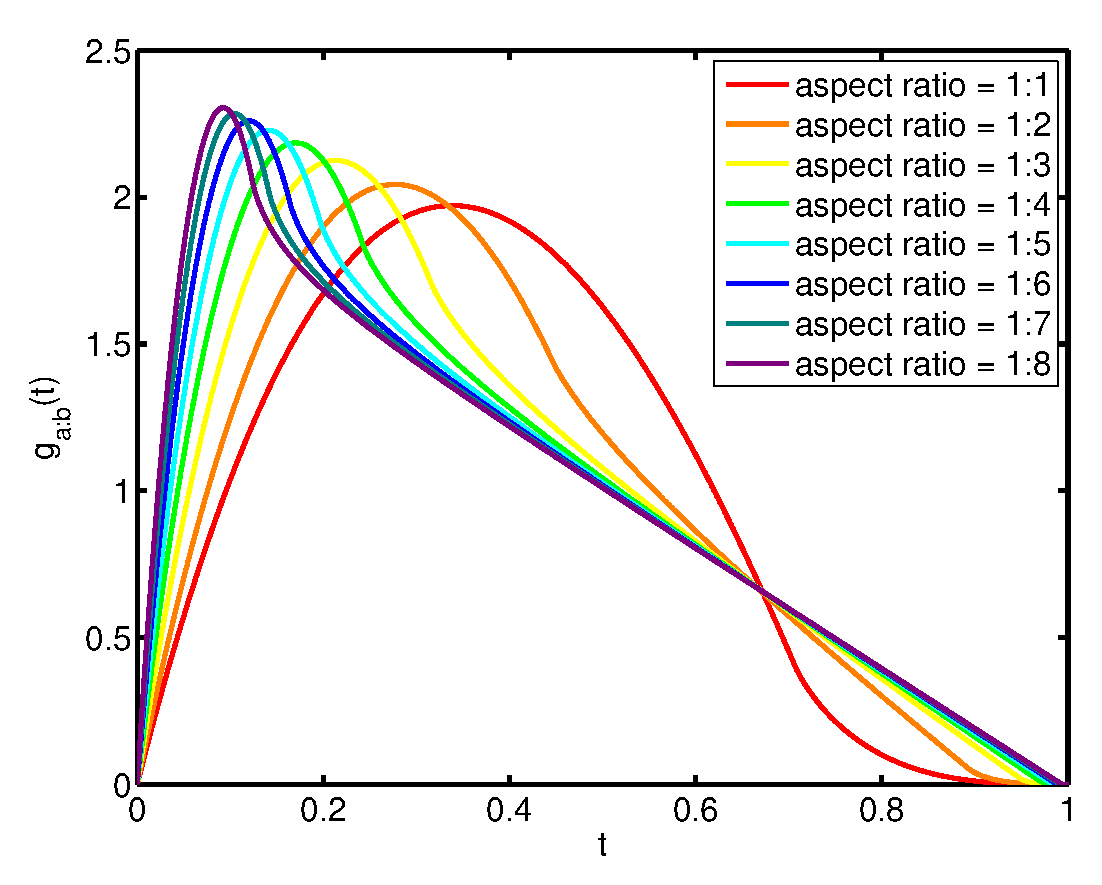
\includegraphics[width=0.33\columnwidth]{../Matlab/Plots/LinePicking_test_rect.eps}}
    \subfloat[\label{fig:b_balls}Density distribution of $n$-D balls.]{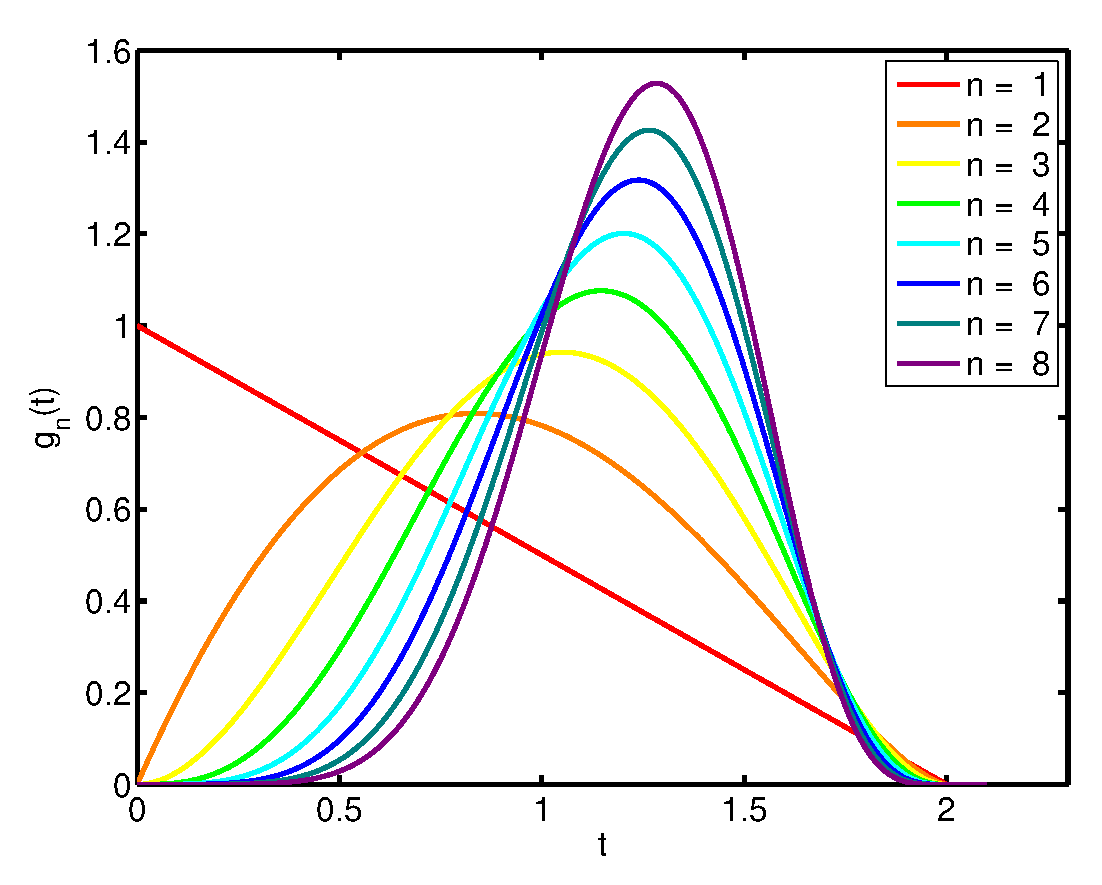
\includegraphics[width=0.33\columnwidth]{../Matlab/Plots/LinePicking_test_balls.eps}}
    \subfloat[\label{fig:various} Various densities distributions for
    shapes with area fixed to 1.]{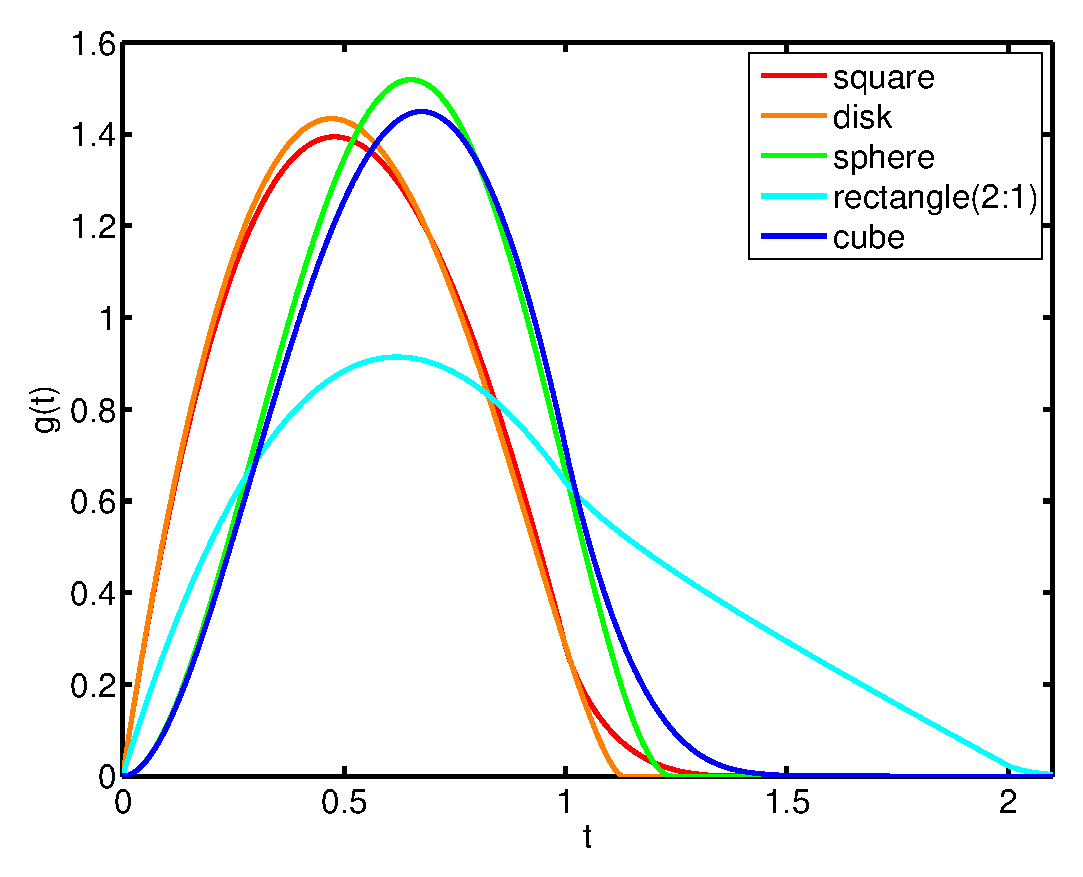
\includegraphics[width=0.33\columnwidth]{../Matlab/Plots/LinePicking_test_fix_area.eps}}
    \caption{Example distance densities.}
  \end{center} 
\vspace{-4mm}
\end{figure}


The other obvious region on which to solve the line-picking problem is
the ball in $n$-dimensions~\cite{tu00:_circle_line} (equations
(27-31)). For a $n$-dimensional ball of radius $R$,
\[ g^{nD-{\rm ball}}_R(t) = n \frac{t^{n-1}}{R^n} I_x\left( 
  \frac{1}{2} (n+1), \frac{1}{2}
                      \right),
\]
where
\[ x = 1 - \frac{t^2}{4 R^2}, \]
and $I_x(p,q)$ is a {\em regularized beta function}
\[  I_x(p,q) = \frac{ B(x; p,q)}{B(p,q)}, \]
where $B(x; p,q)$ is an incomplete beta function, and $B(p,q)$ is a
beta function, i.e., 
\begin{eqnarray*}
  B(p,q)    & = & \int_0^1 t^{p-1} (1 - t)^{q-1} \, dt, \\
  B(x; p,q) & = & \int_0^x t^{p-1} (1 - t)^{q-1} \, dt.
\end{eqnarray*}
The first few of these are \cite{tu00:_circle_line} ($P_2$ in (5) and
(17), $P_3$ in (9) and (19), $P_4$ in (18) and $P_5$ in (20), general
even form in (15), general odd form in (16)):
\begin{eqnarray}
  \label{eq:ball_line_picking}
  g^{1D-{\rm ball}}_R(t) & = & \frac{1}{R} - \frac{t}{2 R}   \label{eq:line_line_picking}, \\
  g^{2D-{\rm ball}}_R(t) & = & \frac{4 t}{\pi R^2} \cos^{-1} \left( \frac{t}{2R} \right)
               - \frac{2 t^2}{\pi R^3} \sqrt{1 - \frac{t^2}{4 R^2} } \label{eq:2dball_line_picking} , \\
          & = & \frac{2 t}{R^2} 
               - \frac{2 t^2}{\pi R^3} \sqrt{1 - \frac{t^2}{4 R^2} }
               - \frac{4 t}{\pi R^2} \sin^{-1} \left( \frac{t}{2R} \right) \label{eq:2dball_line_picking2} ,  \\
  g^{3D-{\rm ball}}_R(t) & = & \frac{3 t^2}{R^3} - \frac{9 t^3}{4 R^4} + \frac{3 t^5}{16 R^6}   \label{eq:sphere_line_picking}  , \\
  g^{4D-{\rm ball}}_R(t) & = &  \frac{8 t^3}{\pi R^4} \cos^{-1} \left( \frac{t}{2R} \right) 
              - \frac{8 t^4}{3 \pi R^5} \left( 1 - \frac{t^2}{4 R^2} \right)^{3/2}
               - \frac{4 t^4}{\pi R^5} \sqrt{1 - \frac{t^2}{4 R^2} } \\
  g^{5D-{\rm ball}}_R(t) & = & \frac{5 t^4}{R^5} - \frac{75 t^6}{16 R^6} + \frac{25 t^7}{32 R^8} - \frac{15 t^9}{256 R^{10}} .
  \label{eq:ball_line_picking-end}
\end{eqnarray}
Tu and Fischbach \cite{tu00:_circle_line} also extend these results to
cases with non-uniform point distributions.
 
Figure~\ref{fig:b_balls} shows a comparison of line picking on
balls of various dimensions, and Figure~\ref{fig:various} shows a
comparison of the 2D and 3D balls to the square and cube. We can see
that as long as the areas (volumes) are matched, they appear quite
similar, respectively, though the rectangle varies considerably more.
% plot is similar to http://mathworld.wolfram.com/BallLinePicking.html




\subsection{Moments}

Ghosh \cite{b.ghosh51:_random_rect} gives the first four moments of
the line-length distribution for the rectangle.
\begin{eqnarray}
  \label{eq:rect_moments} 
  \alpha_1 & = & \frac{1}{6} \left[ 
                        \frac{b^2}{a} \cosh^{-1}\left( M/b \right) +
                        \frac{a^2}{b} \cosh^{-1}\left( M/a \right) 
                 \right]
                  + \frac{1}{15} \left[ \frac{a^3}{b^2} + \frac{b^3}{a^2} \right]
                  - \frac{M}{15} \left[ \frac{a^2}{b^2} + \frac{b^2}{a^2} -3 \right],
\\
  \alpha_2 & = & \frac{1}{6} M^2, \\
  \alpha_3 & = & \frac{1}{20} \left[ 
                        \frac{b^4}{a} \cosh^{-1}\left( M/b \right) +
                        \frac{a^4}{b} \cosh^{-1}\left( M/a \right) 
                 \right]
                  + \frac{2}{105} \left[ \frac{a^5}{b^2} + \frac{b^5}{a^2} \right]
                  - \frac{2M}{105} \left[ \frac{a^4}{b^2} + \frac{b^4}{a^2}\right]
                        - \frac{5}{84} M^3, 
\\
  \alpha_4 & = & \frac{1}{15} a^4 + \frac{1}{18} a^2 b^2 + \frac{1}{15} b^4,
\end{eqnarray}
where $M = \sqrt{a^2 + b^2}$, from which we can derive the special
cases of the square and line (though these can also be derived
directly). Obvious central moments such as mean, and variance, etc.,
can be derived from these, though forumlas will be complex.

The mean for the cube, known as the {\em Robbins constant}, is given
in \cite{robbins78:_constant,weisstein:_cube_line_picking} as
\begin{equation}
   \label{eq:cube_mean}
 \mu^{\rm cube} = \frac{1}{105} \left[ 
                             4 + 17 \sqrt{2}- 6 \sqrt{3}  +
                             21 \ln(1+\sqrt{2}) + 
                             42 \ln(2+\sqrt{3}) - 7 \pi
                      \right]
	=	0.66170...
\end{equation}
but a closed form for the variance does not appear (only even moments
are reported). Even more complicated results appear for 4- and 5-Cubes in
5-Cubes~\cite{philip:_probab_distr_distan_between_two_4d}:
\begin{eqnarray}
 \mu^{\rm 4-cube} & = & 0.7776656535 ...    \label{eq:4-cube}, \\
 \mu^{\rm 4-cube} & = & 0.8785309152 ...     \label{eq:5-cube}.
\end{eqnarray}

The means for the $n$-dimensional ball (with radius 1) are given in
\cite{weisstein:_ball_line_picking} as
\begin{eqnarray}
  \label{eq:ball-ndim-mean}
  \mu^{1D-{\rm ball}} & = & \frac{2}{3}, \\
  \mu^{2D-{\rm ball}} & = & \frac{128}{45 \pi},\\
  \mu^{3D-{\rm ball}} & = & \frac{36}{35}, \\
  \mu^{4D-{\rm ball}} & = & \frac{16384}{4725 \pi}.
\end{eqnarray}
The more general form for higher order moments is given in
\cite{tu00:_circle_line} (equation (138-141)) as
\begin{eqnarray}
  \label{eq:ball-ndim-moments}
  \alpha_m^{nD-{\rm ball}} & = &
     \frac{n 2^{m+n}}{m+n} \frac{B\left(\frac{n+1}{2}, \frac{n+m+1}{2}  \right)}{B\left(\frac{n+1}{2}, \frac{1}{2} \right)} R^m, \\
       & = & \left( \frac{n}{n+m} \right)^2 
                 \frac{\Gamma\left( n+m+1 \right) \Gamma\left( n/2 \right) }
                      {\Gamma\left( (n+m)/2 \right) \Gamma\left( n+1 + m/2 \right) } R^m.  
\end{eqnarray}
for and $n$-dimensional ball of radius $R$.



\subsection{CDF}


Cumulative distribution functions are also known ...

Can be calculated by integration, but ...



\subsection{Approximations}




% In high dimensions, the points are spread ``more thinnly'' in the
% sense that their density on $n$-dimensional volumes will be lower, and
% hence, the distances between points will be larger. As a result,
% Waxman graphs in higher dimensions may become more sparse.






Note that once again we can derive a small $t$ approximation,
namely, 
\[ g_{a,b}(t) \simeq \frac{4 t}{a^2 b^2} \frac{ab \pi}{2}
            = \frac{2 \pi t}{a b} \]
though here we must assume that the scale-length implied by $\alpha$
is smaller than $a$, the minimum dimension of the rectangle.  Once
again, the approximation is the same as that of the rectangle and
disk, with respect to unit area.




The universality of the small $t$ expansions (used for deriving small
$\alpha$ approximations to the length distributiohn) suggests a
general form
\[ g(t) \simeq \frac{2 \pi t}{A} = 2 \pi d, \]
where $A$ is the area of the region of interest and $d$ is the scaled
distance $d = t/A$. Notice that this scaling is different from the one
used in the Waxman distance function where we scale by the maximum
distnace $L$. 

It is also numerically straight-forward to compute $g(t)$ where the
points are placed non-uniformly in the region of interest. Some
analytic cases are treated in \cite{tu00:_circle_line}, but for
instance dealing with an inhomogeneous Poisson process used to model
``burstiness'' or clustering of points, and thence with a somewhat
different structure than the standard Waxman graph.


We also know the asymptotic form of these distributions for $t
\rightarrow 0$, i.e., 
\begin{equation}
  \label{eq:asympt_line_picking}
  g_n(t) \simeq n \frac{t^{n-1}}{R^n}
\end{equation}
because we can write % http://en.wikipedia.org/wiki/Beta_function
\begin{eqnarray*} 
   I_x(a,b) 
& = & \sum_{j=a}^{a+b-1} {(a+b-1)! \over j!(a+b-1-j)!} x^j (1-x)^{a+b-1-j} \\
& = & \sum_{j=a}^{a+b-1} {(a+b-1)! \over j!(a+b-1-j)!} 
        \left(1 - \frac{t^2}{4 R^2}\right)^j \left( \frac{t^2}{4 R^2} \right)^{a+b-1-j} \\
& = & \left(1 - \frac{t^2}{4 R^2}\right)^{a+b-1}
       + \sum_{j=a}^{a+b-2} {(a+b-1)! \over j!(a+b-1-j)!} 
        \left(1 - \frac{t^2}{4 R^2}\right)^j \left( \frac{t^2}{4 R^2} \right)^{a+b-1-j} \\
& = & 1 + O(t),
\end{eqnarray*}
and this is directly useful for calculating large $s$ (small $\alpha$)
approximations of the estimator.

For instance, from before, we know that if the $j$th derivative of
$g(t)$ at $t = 0$ is the first non-zero derivative, then the ratio of
Laplace transforms takes the form $\sim (j+1)/s$, so here, it is
immediately obvious that
\[ -G_n(s)/G_n(s) \rightarrow n/s, \]
for large $s$. 

This result is now obvious for the sphere, but for non-spherical (but
convex) regions, we simply need to consider $s$ large enough that the
probability of links longer than $\epsilon$ is negligable, where
$\epsilon$ is chosen so that the chance of intersecting with a
boundary is negligable, and so we can use a spherical
approximation. For instance, the {\em cube line picking} problem has
probability distribution given by \cite{weisstein:_cube_line_picking},
which has first non-zero term of $O(t)$, which is correct for a 2D
space.

We can extend some of this insight into other problems, for instance,
the {\em circle line picking} problem, where pairs of points are
chosen on a circle, but the lines cross the circle. Here, the
probability distribution for line length (with a unit circle) is
\cite{weisstein:_circle_line_picking}
% http://mathworld.wolfram.com/CircleLinePicking.html
\begin{equation}
  \label{eq:circle_line_picking}
  g(t) = \frac{1}{\pi} \left(    
           1 - \frac{s^2}{4}
               \right)^{-1/2} 
       \simeq \frac{1}{\pi} \left( 1 - \frac{s^2}{4} + \cdots \right) 
\end{equation}
whereas in {\em sphere line
  picking}~\cite{weisstein:_sphere_line_picking}, there distribution
takes the form
\begin{equation}
  \label{eq:sphere_line_picking_approx}
  g(t) = \frac{1}{2} t.
\end{equation}
Clearly in this type of case, the dimension of the space is not the
critical factor, because the space on which the points are chosen is
embedded in a larger space from which lines are chosen, and the
geometry of the relationship is important.


INCIDENTALLY -- limit n -> infty for balls, has almost fixed distances
between nodes, so it approaches ER graph




\section{Numerical Computation by Simulation}
\label{sec:numerical}

It may be possible that one wishes to compute distributions, on
irregular regions, for which there is no closed form solution.
Numerically it is straight-forward to calculate the function
$g(t)$. There are two obvious approaches:
\begin{itemize}

\item Numerical computation of a $n$-dimensional integral over
  $\Omega$, or

\item Simulation of the problem, and estimation of the density from
  simulated results. 

\end{itemize}
The two approaches have different advantages and disadvantages. The
former approach has no stochastic component, and so errors are
predictable and regular. 

The later approach allows complex, potentially non-convex,
non-uniform, problems to be solved as long as they can be
simulated. Given the stochastic nature of the latter, it may help to
say a little more:

The general process is as follows:
\begin{enumerate}

\item Simulate a set of $2N$ points in the region of interest, and
  calculate the distances between successive pairs. The region may be
  irregular, or even non-convex; decisions may be made about some
  lines being inadmissable (because, for instance, they are exterior
  to the region for a non-convex region), or distances may be
  non-Euclidean, or the point distribution can be non-uniform. All
  that is needed is a set of output distances $\{ t_i \}_{i=1}^{N}$.

\item The density could then be approximate through binning, or a
  kernal smoothing technique, but in fact, we don't need direct access
  to the density as the estimator uses the Laplace transform.

\end{enumerate}

We have tested the above approach, running it 30 times (with different
seeds), in Matlab for various values of $N$. The results are shown in
Figure~\ref{fig:simulated_laplace}. The first plot shows estimates of
the mean relative absolute error of the estimated Laplace transforms
over the range $S \in [0, 50]$. We can see from the fitted straight
line, that the errors decrease as $1/\sqrt{N}$, dropping to around 1\%
at around $N=100,000$.


....





The second plot shows the computation times\footnote{Both algorithms
  were implemented in Matlab, the exact method using Matlab's {\tt
    quadqk} function. } relative to the computation times for the
``exact'' method\footnote{Note that both techniques are in some
  respect numerical, because even when we have a closed form solution
  for the density, we still typically need to numerically integrate
  this to obtain the Laplace transform, but we shall refer to this
  solution as ``exact'' for the sake of clarity in the following
  results, and because in the following we perform numerical
  integration with error tolerances of $10^{-6}$, which means the
  errors in this approach are significantly smaller than those of the
  simulation-based approach, at least for the ranges of $N$ tested
  here.}  We can immediately notice that computation times are roughly
linear in $N$, as one might expect. that around the range $N=100,000$,
the simulation approach is competitive with the exact approach.

The simulation-based approach is not as accurate as the exact
numerical approach, however, it accuracy should be sufficient for most
estimation problems, without increasing the computational workload
unduly.

\begin{figure}[tbp]
  \begin{center}
    \subfloat[Mean relative error in $-G'(\hat{s})/G(\hat{s})$.]{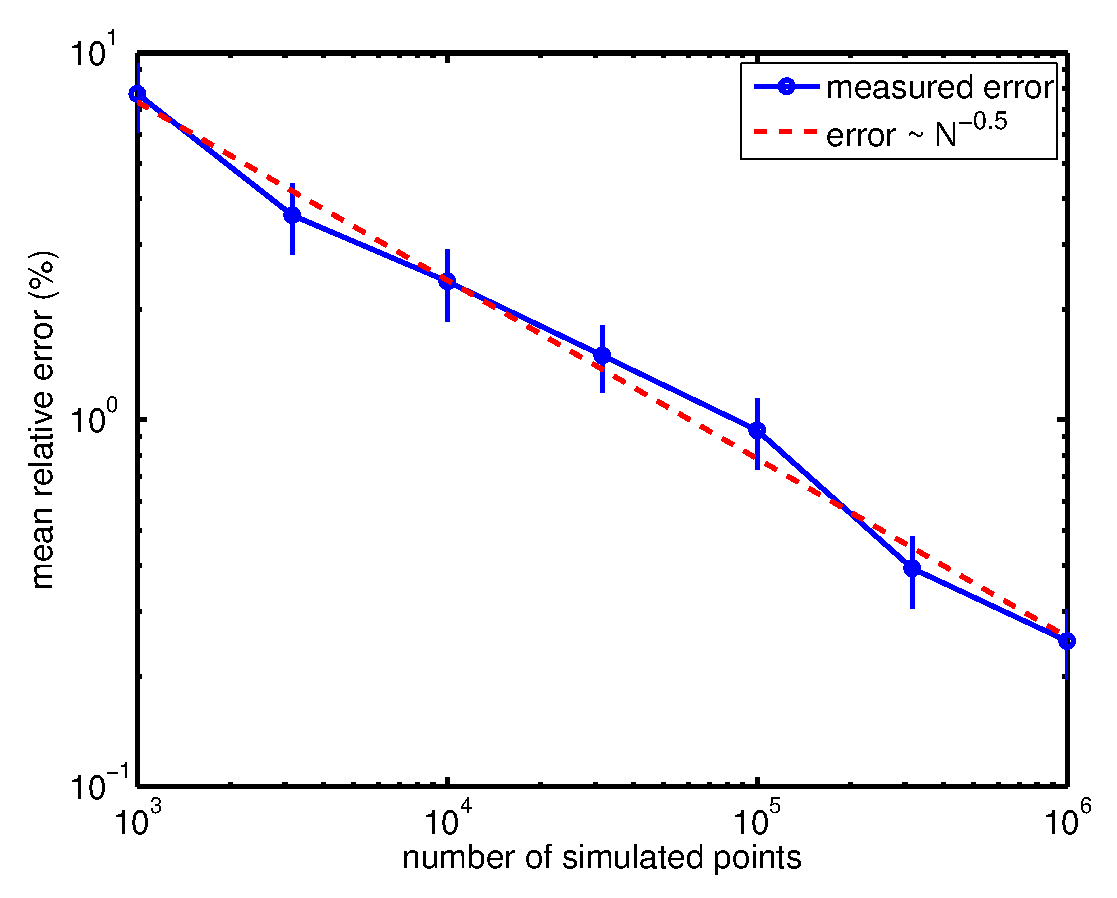
\includegraphics[width=0.49\columnwidth]{../Matlab/Plots/LinePicking_numerical_rel_error.eps}}
    \subfloat[Relative computation time of the simulation-based
    approach, with respect to the exact approach.]{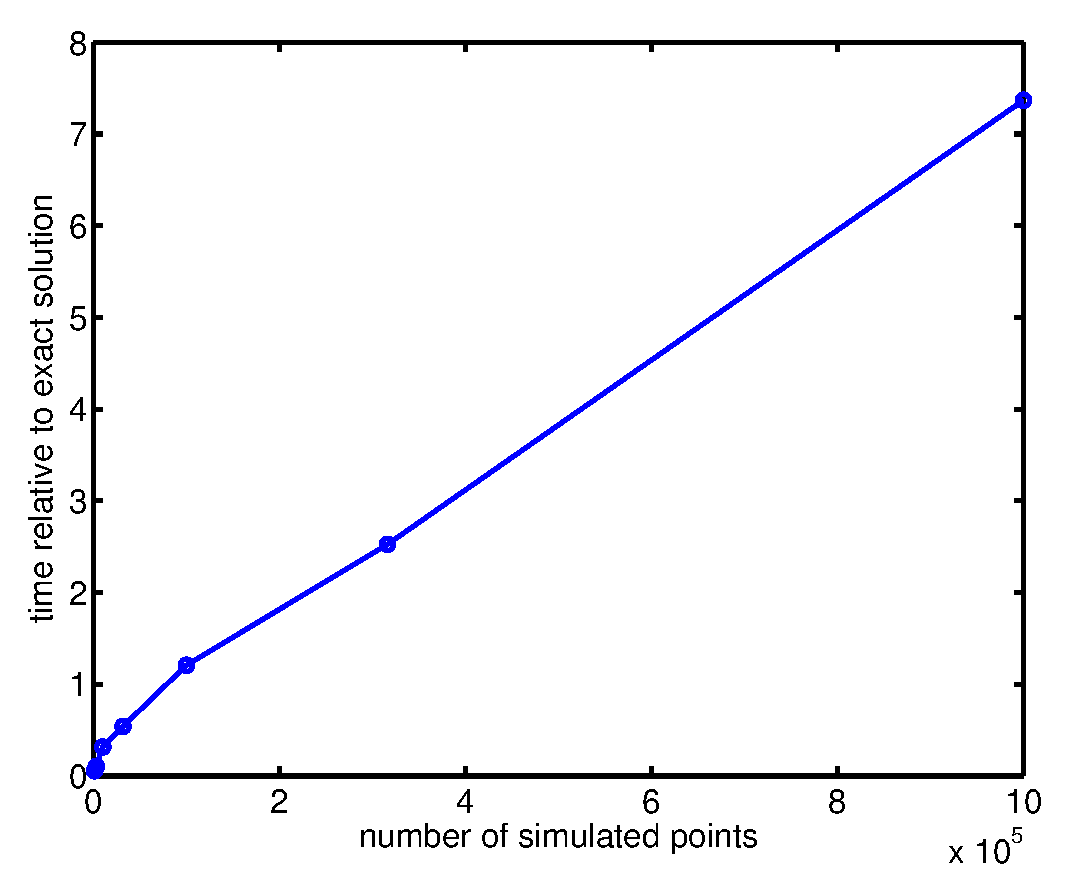
\includegraphics[width=0.49\columnwidth]{../Matlab/Plots/LinePicking_numerical_time.eps}}
    \caption{A comparison of simulation-based Laplace transform
      calculation with the exact approach.\label{fig:simulated_laplace}}
  \end{center} 
\vspace{-4mm}
\end{figure}


\section{Programs}
\label{sec:program}

\subsection{A Rough Guide}

\subsection{Numerical Issues}


\section{Correlations}

Correlations between distances \cite{bartlett64}

(0) correlation between a pair 1/10

(i) $n$ nodes, then $N = n (n-1)/2$ pairs of nodes, and so this many pairs of distances

(ii) the $N (N-1) /2 = n (n-1) (n (n-1) -1)/8 = $ possible pairs of
correlations

(iii) but only $n(n-1)(n-2)/2$ of the correlations are positive,
because they share a node so we get average correlation between all
pairs
 \[ \frac{1}{10} \frac{n(n-1)(n-2)/2}{n (n-1) (n (n-1) -1)/8} =
    \frac{2}{5} \frac{(n-2)}{(n (n-1) -1)}
   \simeq 
   \frac{2}{5n}
\]
for large $n$

Empirical measurement (see triples.m)
\[ r = 0.114865 \pm 0.000037\]


\section{Conclusion and Future Work}




\setlength{\parskip}{1mm}
\bibliographystyle{ieeetr}
% \bibliography{queueing_theory,books,ip_traffic,time_series,reliability,tcp,ospf,lrd,worms,internet,routing,bgp,topology,network,traffic_engineering,algorithms,optimization,history,graph}
\bibliography{LinePicking}

\end{document}


